\subsection{Canny Edge Detection}

Bruger output fra eksempelvis Sobel som input.

\begin{enumerate}
	\item Laver kanterne ''tyndere''. Kanterne kan være spredt ud på mange pixels i et højopløsnings billede. Dette gøres ved at bruge output fra Sobel og tjekke om den aktuelle pixel er mere tydelig end dens nabo. Da vi efter de forskellige Sobel masker ved hvilken origientering denne kant har, kan vi tage højde for det, og derved kun medregne pixels som har en anden gradient end den aktuelle.
	\item \textbf{Hysteresis Thresholding} bruges til yderligere at fjerne udbetydelige kanter. Se Figur~\ref{fig:hysteresis-thresholding}.
\end{enumerate}

\begin{figure}[H]
	\centering
	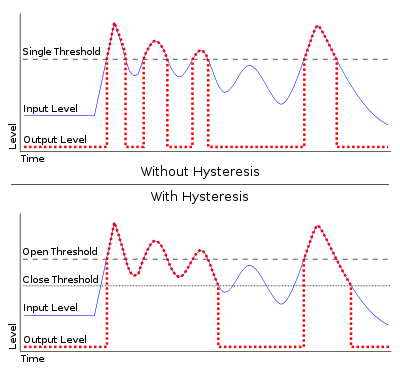
\includegraphics[width=0.7\linewidth]{figs/spm11/hysteresis-thresholding}
	\caption{Eksempel på Hysteresis Thresholding.}
	\label{fig:hysteresis-thresholding}
\end{figure}
